%===============================================================================
% LaTeX sjabloon voor de bachelorproef toegepaste informatica aan HOGENT
% Meer info op https://github.com/HoGentTIN/latex-hogent-report
%===============================================================================

\documentclass[dutch,dit,thesis]{hogentreport}

% TODO:
% - If necessary, replace the option `dit`' with your own department!
%   Valid entries are dbo, dbt, dgz, dit, dlo, dog, dsa, soa
% - If you write your thesis in English (remark: only possible after getting
%   explicit approval!), remove the option "dutch," or replace with "english".

\usepackage{lipsum} % For blind text, can be removed after adding actual content

%% Pictures to include in the text can be put in the graphics/ folder
\graphicspath{{graphics/}}

%% For source code highlighting, requires pygments to be installed
%% Compile with the -shell-escape flag!
\usepackage[section]{minted}
\usemintedstyle{solarized-light}
\definecolor{bg}{RGB}{253,246,227} %% Set the background color of the codeframe

%% Change this line to edit the line numbering style:
\renewcommand{\theFancyVerbLine}{\ttfamily\scriptsize\arabic{FancyVerbLine}}

%% Macro definition to load external java source files with \javacode{filename}:
\newmintedfile[javacode]{java}{
    bgcolor=bg,
    fontfamily=tt,
    linenos=true,
    numberblanklines=true,
    numbersep=5pt,
    gobble=0,
    framesep=2mm,
    funcnamehighlighting=true,
    tabsize=4,
    obeytabs=false,
    breaklines=true,
    mathescape=false
    samepage=false,
    showspaces=false,
    showtabs =false,
    texcl=false,
}

% Other packages not already included can be imported here

%%---------- Document metadata -------------------------------------------------
% TODO: Replace this with your own information
\author{Ernst Aarden}
\supervisor{Dhr. F. Van Houte}
\cosupervisor{Mevr. S. Beeckman}
\title[Optionele ondertitel]%
    {Titel van de bachelorproef}
\academicyear{\advance\year by -1 \the\year--\advance\year by 1 \the\year}
\examperiod{1}
\degreesought{\IfLanguageName{dutch}{Professionele bachelor in de toegepaste informatica}{Bachelor of applied computer science}}
\partialthesis{false} %% To display 'in partial fulfilment'
%\institution{Internshipcompany BVBA.}

%% Add global exceptions to the hyphenation here
\hyphenation{back-slash}

%% The bibliography (style and settings are  found in hogentthesis.cls)
\addbibresource{bachproef.bib}            %% Bibliography file
\addbibresource{../voorstel/voorstel.bib} %% Bibliography research proposal
\defbibheading{bibempty}{}

%% Prevent empty pages for right-handed chapter starts in twoside mode
\renewcommand{\cleardoublepage}{\clearpage}

\renewcommand{\arraystretch}{1.2}

%% Content starts here.
\begin{document}

%---------- Front matter -------------------------------------------------------

\frontmatter

\hypersetup{pageanchor=false} %% Disable page numbering references
%% Render a Dutch outer title page if the main language is English
\IfLanguageName{english}{%
    %% If necessary, information can be changed here
    \degreesought{Professionele Bachelor toegepaste informatica}%
    \begin{otherlanguage}{dutch}%
       \maketitle%
    \end{otherlanguage}%
}{}

%% Generates title page content
\maketitle
\hypersetup{pageanchor=true}

%%=============================================================================
%% Voorwoord
%%=============================================================================

\chapter*{\IfLanguageName{dutch}{Woord vooraf}{Preface}}%
\label{ch:voorwoord}

Deze bachelorproef is geschreven in het kader van mijn opleiding Bachelor in de Toegepaste Informatica aan de Hogeschool Gent. Dit onderzoek is toegewezen door docent Lena De Mol en sprak mij meteen aan vanwege het innovatieve idee van Zorglab 360°. De mogelijkheid om mee te helpen aan een nieuwe vorm van therapie leek mij dan ook zeer interessant.\\

Dit onderzoek had echter niet tot stand kunnen komen zonder de hulp van verschillende mensen, waarvoor ik enorm dankbaar ben.\\

Allereerst wil ik mijn promotor, Stijn Lievens, bedanken voor de waardevolle feedback die ik heb ontvangen tijdens het schrijven van deze bachelorproef. Hij heeft mij altijd goed advies gegeven en heeft ook bijgedragen aan de sturing van mijn onderzoek.\\

Daarnaast wil ik ook mijn co-promotor, Jana Van Damme, bedanken voor het introduceren van het onderzoek en haar inspanningen om het onderzoek te begrijpen. Ondanks dat zij misschien niet over de technische expertise beschikt, heeft zij altijd haar best gedaan om alles zo goed mogelijk te begrijpen en mij duidelijk uit te leggen wat er onderzocht moest worden.\\

Tot slot wil ik mijn ouders bedanken voor hun financiële steun bij het volgen van deze studierichting.\\

Ik wens u veel leesplezier toe en hoop dat dit onderzoek leidt tot iets innovatiefs.
%%=============================================================================
%% Samenvatting
%%=============================================================================

% TODO: De "abstract" of samenvatting is een kernachtige (~ 1 blz. voor een
% thesis) synthese van het document.
%
% Een goede abstract biedt een kernachtig antwoord op volgende vragen:
%
% 1. Waarover gaat de bachelorproef?
% 2. Waarom heb je er over geschreven?
% 3. Hoe heb je het onderzoek uitgevoerd?
% 4. Wat waren de resultaten? Wat blijkt uit je onderzoek?
% 5. Wat betekenen je resultaten? Wat is de relevantie voor het werkveld?
%
% Daarom bestaat een abstract uit volgende componenten:
%
% - inleiding + kaderen thema
% - probleemstelling
% - (centrale) onderzoeksvraag
% - onderzoeksdoelstelling
% - methodologie
% - resultaten (beperk tot de belangrijkste, relevant voor de onderzoeksvraag)
% - conclusies, aanbevelingen, beperkingen
%
% LET OP! Een samenvatting is GEEN voorwoord!

%%---------- Nederlandse samenvatting -----------------------------------------
%
% TODO: Als je je bachelorproef in het Engels schrijft, moet je eerst een
% Nederlandse samenvatting invoegen. Haal daarvoor onderstaande code uit
% commentaar.
% Wie zijn bachelorproef in het Nederlands schrijft, kan dit negeren, de inhoud
% wordt niet in het document ingevoegd.

\IfLanguageName{english}{%
\selectlanguage{dutch}
\chapter*{Samenvatting}
\lipsum[1-4]
\selectlanguage{english}
}{}

%%---------- Samenvatting -----------------------------------------------------
% De samenvatting in de hoofdtaal van het document

\chapter*{\IfLanguageName{dutch}{Samenvatting}{Abstract}}

\lipsum[1-4]


%---------- Inhoud, lijst figuren, ... -----------------------------------------

\tableofcontents

% In a list of figures, the complete caption will be included. To prevent this,
% ALWAYS add a short description in the caption!
%
%  \caption[short description]{elaborate description}
%
% If you do, only the short description will be used in the list of figures

\listoffigures

% If you included tables and/or source code listings, uncomment the appropriate
% lines.
%\listoftables
%\listoflistings

% Als je een lijst van afkortingen of termen wil toevoegen, dan hoort die
% hier thuis. Gebruik bijvoorbeeld de ``glossaries'' package.
% https://www.overleaf.com/learn/latex/Glossaries

%---------- Kern ---------------------------------------------------------------

\mainmatter{}

% De eerste hoofdstukken van een bachelorproef zijn meestal een inleiding op
% het onderwerp, literatuurstudie en verantwoording methodologie.
% Aarzel niet om een meer beschrijvende titel aan deze hoofdstukken te geven of
% om bijvoorbeeld de inleiding en/of stand van zaken over meerdere hoofdstukken
% te verspreiden!

%%=============================================================================
%% Inleiding
%%=============================================================================

\chapter{\IfLanguageName{dutch}{Inleiding}{Introduction}}%
\label{ch:inleiding}

De inleiding moet de lezer net genoeg informatie verschaffen om het onderwerp te begrijpen en in te zien waarom de onderzoeksvraag de moeite waard is om te onderzoeken. In de inleiding ga je literatuurverwijzingen beperken, zodat de tekst vlot leesbaar blijft. Je kan de inleiding verder onderverdelen in secties als dit de tekst verduidelijkt. Zaken die aan bod kunnen komen in de inleiding~\autocite{Pollefliet2011}:

\begin{itemize}
  \item context, achtergrond
  \item afbakenen van het onderwerp
  \item verantwoording van het onderwerp, methodologie
  \item probleemstelling
  \item onderzoeksdoelstelling
  \item onderzoeksvraag
  \item \ldots
\end{itemize}

\section{\IfLanguageName{dutch}{Probleemstelling}{Problem Statement}}%
\label{sec:probleemstelling}

Uit je probleemstelling moet duidelijk zijn dat je onderzoek een meerwaarde heeft voor een concrete doelgroep. De doelgroep moet goed gedefinieerd en afgelijnd zijn. Doelgroepen als ``bedrijven,'' ``KMO's'', systeembeheerders, enz.~zijn nog te vaag. Als je een lijstje kan maken van de personen/organisaties die een meerwaarde zullen vinden in deze bachelorproef (dit is eigenlijk je steekproefkader), dan is dat een indicatie dat de doelgroep goed gedefinieerd is. Dit kan een enkel bedrijf zijn of zelfs één persoon (je co-promotor/opdrachtgever).

\section{\IfLanguageName{dutch}{Onderzoeksvraag}{Research question}}%
\label{sec:onderzoeksvraag}

Wees zo concreet mogelijk bij het formuleren van je onderzoeksvraag. Een onderzoeksvraag is trouwens iets waar nog niemand op dit moment een antwoord heeft (voor zover je kan nagaan). Het opzoeken van bestaande informatie (bv. ``welke tools bestaan er voor deze toepassing?'') is dus geen onderzoeksvraag. Je kan de onderzoeksvraag verder specifiëren in deelvragen. Bv.~als je onderzoek gaat over performantiemetingen, dan 

\section{\IfLanguageName{dutch}{Onderzoeksdoelstelling}{Research objective}}%
\label{sec:onderzoeksdoelstelling}

Wat is het beoogde resultaat van je bachelorproef? Wat zijn de criteria voor succes? Beschrijf die zo concreet mogelijk. Gaat het bv.\ om een proof-of-concept, een prototype, een verslag met aanbevelingen, een vergelijkende studie, enz.

\section{\IfLanguageName{dutch}{Opzet van deze bachelorproef}{Structure of this bachelor thesis}}%
\label{sec:opzet-bachelorproef}

% Het is gebruikelijk aan het einde van de inleiding een overzicht te
% geven van de opbouw van de rest van de tekst. Deze sectie bevat al een aanzet
% die je kan aanvullen/aanpassen in functie van je eigen tekst.

De rest van deze bachelorproef is als volgt opgebouwd:

In Hoofdstuk~\ref{ch:stand-van-zaken} wordt een overzicht gegeven van de stand van zaken binnen het onderzoeksdomein, op basis van een literatuurstudie.

In Hoofdstuk~\ref{ch:methodologie} wordt de methodologie toegelicht en worden de gebruikte onderzoekstechnieken besproken om een antwoord te kunnen formuleren op de onderzoeksvragen.

% TODO: Vul hier aan voor je eigen hoofstukken, één of twee zinnen per hoofdstuk

In Hoofdstuk~\ref{ch:conclusie}, tenslotte, wordt de conclusie gegeven en een antwoord geformuleerd op de onderzoeksvragen. Daarbij wordt ook een aanzet gegeven voor toekomstig onderzoek binnen dit domein.
\chapter{\IfLanguageName{dutch}{Stand van zaken}{State of the art}}%
\label{ch:stand-van-zaken}

% Tip: Begin elk hoofdstuk met een paragraaf inleiding die beschrijft hoe
% dit hoofdstuk past binnen het geheel van de bachelorproef. Geef in het
% bijzonder aan wat de link is met het vorige en volgende hoofdstuk.

% Pas na deze inleidende paragraaf komt de eerste sectiehoofding.

In dit hoofdstuk wordt de stand van zaken behandeld, ook wel \emph{state of the art} genoemd. Het doel van dit hoofdstuk is om u een overzicht te geven van de meest recente kennis en ontwikkelingen binnen ASR-modellen en machine learning met betrekking tot spraakherkenning. In dit gedeelte wordt voornamelijk ingegaan op modellen en hun werking. Bovendien wordt de relevante terminologie verduidelijkt en uitgelegd. Dit state-of-the-art overzicht biedt de lezer een solide basis om de verdere ontwikkelingen en resultaten in dit onderzoek te begrijpen.
\section{Automatic Speech Recognition}
Automatic speech recognition (ASR) is een technologie die spraakaudio omzet in tekst. Zo bestaan er dan ASR-modellen die de audio analyseren en deze omzetten in een reeks woorden die overeenkomen met wat er werd gezegd. ASR-systemen worden al in verschillende toepassingen gebruikt, namelijk chatbots, automatische translaties in video's en nog veel meer.\autocite{Microsoft2017} Modellen worden getraind met behulp van grote datasets gesproken taal en kunnen daarna geoptimaliseerd worden voor specifieke talen en taken. Gaandeweg zijn er veel kern technologieën ontwikkeld, zoals Gaussiaanse Mixture Models (GMM's), verborgen Markov-modellen (HMM's), mel-frequentie cepstrale coëfficiënten (MFCC's) en hun afgeleiden, ngram-taalmodellen (LM's), discriminerende training. Dit zijn een hele boel technieken die de stand-van-zaken op gebied van ASR enorm verbeterd hebben.\autocite{Mahesha2016}

\subsection{Word Error Rate}
Word Error Rate (WER) is een belangrijke maateenheid die wordt gebruikt om de nauwkeurigheid van ASR-systemen te evalueren. WER is afgeleid van de $\emph{Levenshtein-afstand}$, ook wel bekend als de $\emph{edit distance}$, die de minimale afstand berekent die nodig is om een reeks woorden om te zetten in een andere reeks woorden door middel van toevoegingen, verwijderingen en substituties van woorden. Bij het evalueren van de nauwkeurigheid van een ASR-systeem wordt de WER berekend als de Levenshtein-afstand tussen een gerefereerd woord en zijn automatische transcriptie, genormaliseerd door de lengte van de reeks referentiewoorden. Dit betekent dat de WER de fouten in het automatische transcriptieproces meet als een percentage van het totale aantal woorden in de referentie-uitvoer. Een lage WER duidt op een hoge nauwkeurigheid van het ASR-systeem, terwijl een hoge WER betekent dat er meer fouten zijn opgetreden tijdens het transcriptieproces \autocite{mccowan2004use}. Door gebruik te maken van de WER als evaluatiemaatstaf kan worden bepaald hoe goed een ASR-systeem presteert en kunnen er verbeteringen worden aangebracht om de nauwkeurigheid van het systeem te verbeteren. \\

De definitie van WER gaat als volgt: $N_r$ zijn de totale woorden in de referentie transcriptie, $N_a$ zijn de totale woorden in de transcriptie, S is het aantal vervangen woorden in de automatische transcriptie, D als het aantal woorden uit de referentie verwijderd in de automatische transcriptie, I is het aantal woorden die in de automatische transcriptie zijn ingevoegd en niet in de referentie voorkomen en H als het aantal correct herkende woorden. Zo kunnen we dan de woord error rate definiëren als: \par 
\[WER = \frac{S + D + I}{N_r}.\]
Dit wordt het meest gebruikt als error verhouding, je kunt aan de hand van WER ook de word recognition rate (WRR) bereken: \par
\[WRR = 1 - WER = \frac{H-I}{N_r} .\]
Soms wordt er ook gebruik gemaakt van de word correct rate (WCR), deze maateenheid maakt geen gebruik van inserties en errors en wordt gedefinieerd als volgt: \par
\[WCR = \frac{H}{N_r} .\] \autocite{mccowan2004use}  
Verduidelijking aan de hand van een voorbeeld: 
\begin{quote}
    Referentietekst: "Het is een zonnige dag vandaag."\\
    Herkende tekst: "Het is een regenachtige dag vandaag."
\end{quote}
Nu wordt er berekend hoe veel invoegingen (I), verwijderingen (D) en substituties (S) er nodig zijn om da herkende tekst overeen te laten komen met de referentietekst:
\begin{quote}
Invoegingen (I): Geen\\
Verwijderingen (D): Geen\\
Substituties (S): `regenachtig' in plaats van 'zonnige'
\end{quote}
Het totale aantal woorden ($N_r$) is 6, dus als we dan de formule volgen ziet dit er als volgt uit:
\[WER = \frac{S + D + I}{N_r} = \frac{1+0+0}{6}.\]
\[WER ≈ 0.1667\]
In dit voorbeeld wordt er een word error rate van ongeveer 0.1667 berekend. Dit wil zeggen dan 16.67\% van de woorden in de herkende tekst afwijkt van de referentietekst.
\subsection{Self-supervised Learning}
In het domein machine learning is self-supervised learning naar voren gekomen als een paradigma om algemene gegevens te leren. Normaal gesproken wordt bij supervised training gebruik gemaakt van data dat gelabeld is. Het probleem is dat ook al is er veel beschikbare data, je kunt pas gebruik maken van supervised learning als deze data gelabeld is. Bij self-supervised learning worden de labels zelf gegenereerd waardoor er geen door mensen geannoteerde labels nodig zijn \autocite{Jaiswal2021}. ASR-systemen zoals Whisper en Wav2Vec gebruik maken van  self-supervised learning. Waardoor het mogelijk wordt gebruik te maken van de grote hoeveelheid ongelabelde gegevens die beschikbaar zijn.

\subsection{Whisper}
Whisper is een ASR-systeem dat in 2022 werd ontwikkeld door OpenAI.
Het is getraind op 680.000 uur aan meertalige gegevens die via het internet zijn verzameld. Door gebruik te maken van grote en diverse data leidt tot verbeterde robuustheid voor accenten, achtergrondgeluiden en technisch taalgebruik\autocite{OpenAI2022}. Om deze reden zou Whisper een geschikte ASR-systeem kunnen zijn voor dit onderzoek.

\subsubsection{Whisper structuur}
De architectuur van Whisper heeft een end-to-end benadering, geïmplementeerd als encoder-decoder transformer. De ingevoerde audio wordt opgesplitst in stukken van 30 seconden. Deze stukken worden dan omgezet in een log-Mel-spectogram wat vervolgens wordt doorgegeven aan een encoder, op figuur \ref{fig:spec} ziet u een voorbeeld van een log-Mel spectogram. Veder gaat dan een getrainde decoder de corresponderende tekstonderschrift voorspellen \autocite{OpenAI2022}. Op figuur \ref{fig:whisp} is een duidelijk overzicht weergegeven van de structuur van Wisper.
\begin{center}
    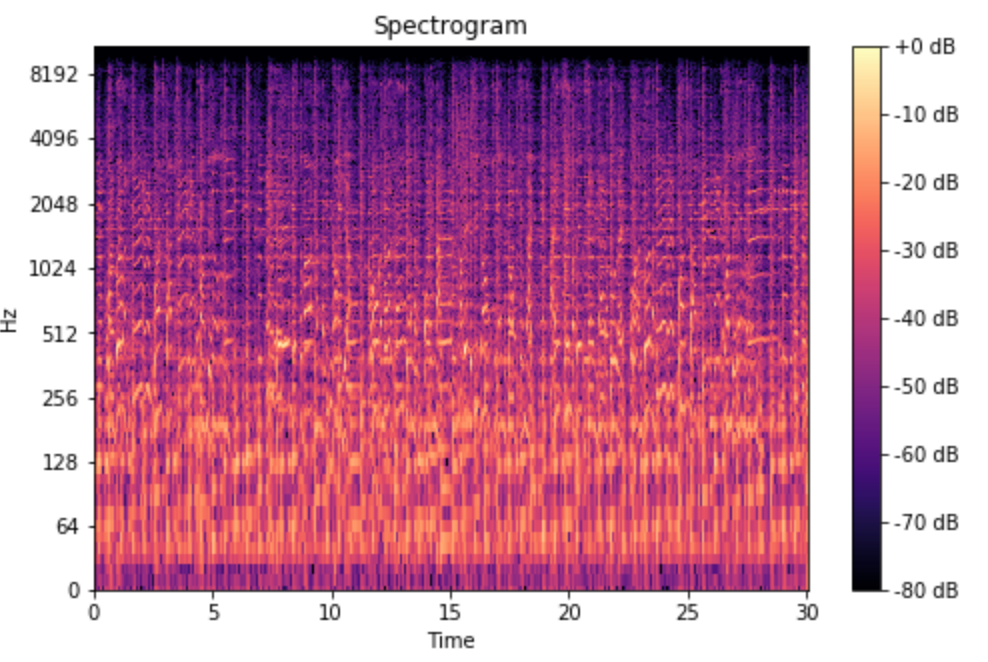
\includegraphics[scale=0.25]{logMelSpec}
    \captionof{figure}{Voorbeeld van een log-mel spectogram, dit geeft een signaal weer op een frequentiespectrum. \autocite{mel-spectrogram-medium}}
    \label{fig:spec}
\end{center}
\begin{center}
    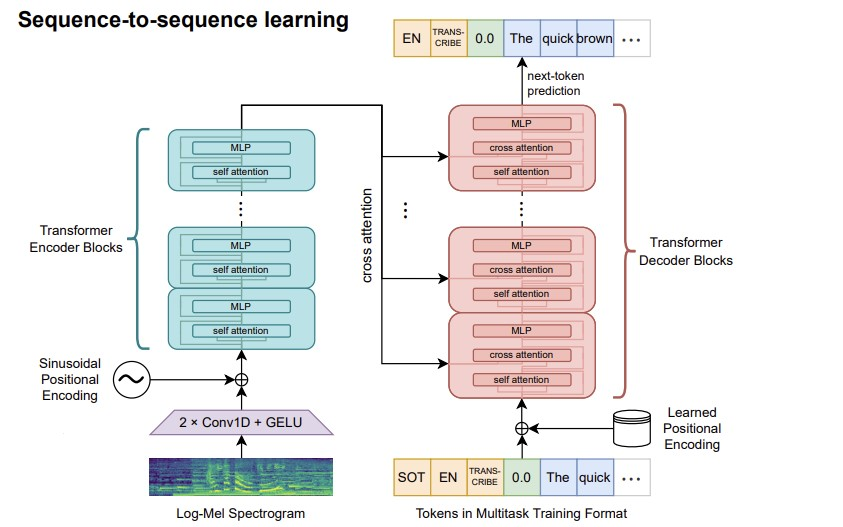
\includegraphics[scale=0.75]{whisper}
    \captionof{figure}{Overzicht van de structuur van het Whisper asr-systeem. \autocite{Tjandra2020}}
    \label{fig:whisp}
\end{center}

\subsubsection{Nederlandse taal}
Whisper is in staat om meerdere talen te begrijpen, waaronder het Nederlands. Whisper heeft verschillende modellen van verschillende groottes, en de prestaties kunnen sterk variëren tussen deze modellen. Het Whisper large-v2-model presteert het beste voor de Nederlandse taal. Bij de Common Voice 9-dataset behaalt het een WER van 5,8\% en bij de Librispeech-dataset een WER van 9,3\% \autocite{Tjandra2020}.

\subsection{Wav2Vec 2.0}
Wav2Vec 2.0 is een framework voor spraakherkenning dat is gemaakt door Facebook AI Research (FAIR). Het is heel populair geworden in de ASR-wereld omdat het heel opmerkelijke prestaties levert. De reden waarom Wav2Vec 2.0 zo goed presteert is omdat het framework zich richt op de raw waveform van de spraak \autocite{baevski2020wav2vec}. Dus in plaats van de audio om te zetten werken ze rechtstreeks met de audio van spraaksignalen. 

\subsubsection{Wav2Vec 2.0 structuur}
Het model is samengesteld uit een Convolutional Neutral Network (CNN), ook wel de feature encoder genoemd, die de raw onbewerkte audio (X) neemt en het levert van latente spraakrepresentaties (z1, z2, ..., zT) voor T tijdsstappen. Vervolgens worden deze dan gevoerd aan een transformer. Deze transformer maakt dan representaties (c1, c2, ..., cT), bij deze stap wordt er ook informatie uit de gehele sequentie vastgelegd. De output van de feature encoder wordt dan gediscretiseerd met een quantization module om het representeren van een doel in het self-supervised learning \autocite{baevski2020wav2vec}. In figuur \ref{fig:wav2vec} zie je een visueel beeld van de structuur van het Wav2Vec 2.0 model.

\begin{center}
    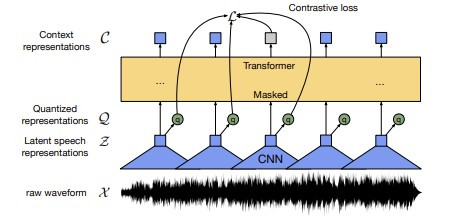
\includegraphics{Wav2Vec}
    \captionof{figure}{Visuele illustratie van de Wav2Vec 2.0 structuur \autocite{baevski2020wav2vec}.}
    \label{fig:wav2vec}
\end{center}

\subsubsection{Performantie}
Natuurlijk wanneer je een spraakherkenningsmodel wilt gebruiken moet je ook kijken naar de prestatie die het kan leveren. Wanneer Wav2Vec 2.0 getest wordt op de LibriSpeech dataset dan krijgen we goede resultaten weer. Bij de 10 minuten gelabelde data presteert het een Word Error Rate (WER) van 4.8\% en bij ongelabelde is het 8.2\%. Hiervoor moest het model natuurlijk eens getraind worden, dit werd gedaan door het 53 duizend uur ongelabelde data van de LibriVox dataset \autocite{baevski2020wav2vec}. 

\subsubsection{Nederlands model}
Wav2vec2-large-xlsr-53-dutch is gemaakt door Jonatas Grosman, een professor aan de katholieke universiteit van Rio de Janeiro. Zijn model is getest geweest met de Common Voice dataset en Collection of Single Speeker (CSS) dataset. Op deze datasets behaalde het een WER van 15.72\% \autocite{grosman2021xlsr53-large-dutch}.\\
Het maakt gebruik van XLSR, een taalmodel is dat gemaakt door Huggingface en Facebook \autocite{2022}. Het doel hiervan is om modellen te trainen die meerdere talen begrijpen en te kunnen verwerken. In tegenstelling tot traditionele taalmodellen, die meestal getraind zijn op één taal, kunnen XLSR-modellen meerdere talen bevatten en kunnen worden afgestemd op een specifieke talen om zo de prestatie van die talen te verbeteren \autocite{2021}.

\section{Stotter Correctie}
Wanneer iemand een ASR model gebruikt en onvloeiend spreekt dan heeft het model moeite met het correct te transcriberen. Gelukkig kan er gebruikt worden van stotter correctie. In 2020 hebben studenten van PES University in India een automatische correctie methode van onvloeibare spraak uitgewerkt. Er wordt gebruik gemaakt van Mel Frequency Cepstral Coefficients (MFCC) en Linear Predictive Coefficients \autocite{KN2020}.

\subsection{Mel Frequency Cepstral Coefficients}
Mel Frequency Cepstral Coefficients is een concept voor het extraheren van kenmerken van een akoestisch signaal. Het is gebaseerd op de frequenties van meer dan 1KHz, dus wat het menselijk gehoor niet meer kan waarnemen. De berekeningen die door MFCC worden uitgevoerd zijn zeer afhankelijk van het proces waarbij de signalen veranderen van analoog naar digitaal. MFCC voert berekeningen uit variërend van de lengte van de golfhoogte, ruis en andere dingen zodat de woorden die werden uitgesproken door de gebruiker worden verkregen \autocite{haq2020speech}.

\subsection{Linear Predictive Coefficients}
Linear Predictive Coding (LPC) is een techniek die wordt gebruikt in audioprocessing en spraakanalyse om de spectrale eigenschappen van een signaal te modelleren. De techniek is gebaseerd op het idee dat het spectrum van een signaal kan worden voorspeld door gebruik te maken van een lineair voorspellingsmodel. Bij LPC wordt het signaal opgedeeld in korte stukjes en wordt er voor elk stukje een set lineaire predictieve coëfficiënten berekend. Deze coëfficiënten worden gebruikt om een lineair voorspellingsmodel te bouwen, dat vervolgens kan worden gebruikt om het spectrum van het signaal te modelleren en te analyseren. De LPC-techniek wordt veel gebruikt in spraaktechnologie, bijvoorbeeld om spraak te comprimeren of om spraak te herkennen in een spraakherkenningssysteem. Het is ook een belangrijk onderdeel van codecs zoals MP3 en AAC, die worden gebruikt voor het comprimeren van audiobestanden. \autocite{bradbury2000linear}. 
 
\subsection{Design}
Het design bestaat uit een sequentie van drie algoritmen. Het eerste algoritme is voor het verwijderen van herhaling, dus worden alle gerepeteerde woorden geëlimineerd en behoudt alle niet-herhaalde woorden. Dit wordt behaald door gebruik MFCC- en LPC-functies van 2 opeenvolgende woorden te extraheren. Als er dan een hoge correlatie is tussen de geëxtraheerde kenmerken van de 2 woorden duidt op een grote gelijkenis tussen woorden, waarna het herhaalde woord wordt geëlimineerd.\\

Er is ook een algoritme voor het verwijderen van lange pauzes in de audio. Dit wordt gedaan door het berekenen van de tijd tussen het einde van een woord en het begin van het opeenvolgende woord. Wanneer dit dan meer dan 0.5s is impliceert dit op een lange pauze.\\

Uiteindelijk is er dan ook een verlenging verwijdering aan de hand van een algoritme. Hierbij wordt het audio fragment opgedeeld in in frames van 50ms. Dan wordt er rekening gehouden met de MFCC- en LPC-kenmerken die overeenkomen met opeenvolgende frames en wordt er een correlatiefactor gevonden. Deze factor wordt achterhaald tussen kenmerken van opeenvolgende frames. Bij een langdurig optreden van hoge correlatie tussen frames impliceert dit dat er een verlenging is (bijvoorbeeld: sttttttttop) \autocite{KN2020}.

\subsection{Performantie}
De algortimen zijn effectief in staat om lange pauzes, verlengingen en herhalingen te herkennen en te corrigeren. Bij de 80 instanties van lange pauzes heeft het algoritme 78 keer de pauzes herkend, dat is een accuraatheid van 97.5\%. Bij het testen op herkenning van verlengingen en herhalingen bevatte de audiobestanden in totaal 60 herhalings- en 70 verlengingsgebeurtenissen. Hierbij werden 2 verschillende functies gebruikt: MFFC en LPC. In figuur \ref{fig:tabel} kunt u zien dat MFCC accurater is dan LPC. MFCC behaalde een gemiddelde nauwkeurigheid van 92.8\% en LPC een 89.9\% \autocite{KN2020}

\begin{center}
    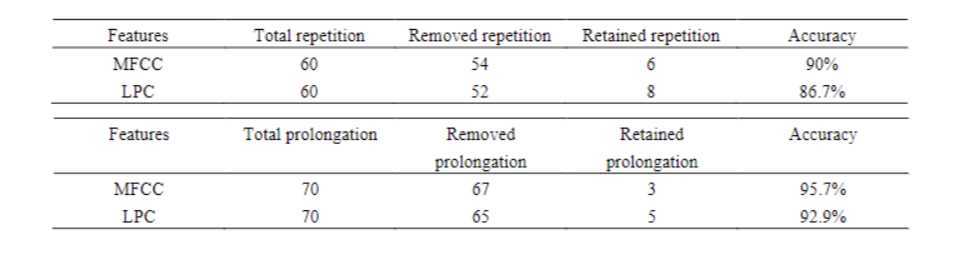
\includegraphics[width = 5in]{tabellen_MFCC_LPC}
    \captionof{figure}{Tabel dat overzicht geef over de accuraatheid van de functies (MFCC, LPC). \autocite{KN2020} }
    \label{fig:tabel}
\end{center}
 
%%=============================================================================
%% Methodologie
%%=============================================================================

\chapter{\IfLanguageName{dutch}{Methodologie}{Methodology}}%
\label{ch:methodologie}

%% TODO: Hoe ben je te werk gegaan? Verdeel je onderzoek in grote fasen, en
%% licht in elke fase toe welke stappen je gevolgd hebt. Verantwoord waarom je
%% op deze manier te werk gegaan bent. Je moet kunnen aantonen dat je de best
%% mogelijke manier toegepast hebt om een antwoord te vinden op de
%% onderzoeksvraag.

Dit hoofdstuk bespreekt hoe het onderzoek zal worden aangepakt. Er worden verschillende aspecten besproken om het uiteindelijke doel te bereiken: het onderzoeken van de theoretische mogelijkheid om stottertherapie in virtual reality te ontwikkelen. Een proof-of-concept zal worden opgesteld om te beoordelen of ASR-systemen stotteraars kunnen begrijpen met behulp van audio-bewerkingsfuncties

\section{Dataset}
De eerste fase in een onderzoek met machine learning is opzoek gaan naar geschikte data. De data moet natuurlijk relevant zijn voor het onderzoek, dus wat er nodig is zijn de audiofragmenten van mensen die stotteren. Daarnaast moet er ook nog voldoende data zijn om duidelijke conclusies te kunnen trekken. Mocht er te weinig data zijn dan is er een mogelijkheid dat de resultaten van het onderzoek afwijken van de realiteit. Ten slotte zou er ook genoeg variatie in de gegevens moeten zitten, want anders zijn de onderzoeken uitgevoerd op één bepaalde toepassing, wordt ook wel \emph{overfitting} genoemd.\\

Voor het samenstellen van de dataset werd gezocht naar audio van personen die stotteren. Podcasts bleken hiervoor een goede bron te zijn en waren gemakkelijk te vinden op platforms zoals YouTube. Om voldoende variatie in de dataset te garanderen, bevat deze zowel audio van een man als van een vrouw. Een van de personen wiens audio in de dataset is opgenomen, is Charlotte Roggeman. Ze heeft haar hele leven last gehad van stotteren, wat relevant is voor dit onderzoek. De andere persoon in de dataset is Rowan Amatkario. Hij heeft sinds zijn jeugd last van stotteren en stottert nog steeds.\\

Naast de audiofragmenten moet er ook een transcriptie zijn per fragment, dit bestaat uit een eenvoudig CSV-bestand. Dit bestand is opgedeeld in 2 kolommen. De eerste kolom is het pad naar de audio file en de tweede kolom is de transcriptie ervan. Transcriptie is een nood omdat dit een manier biedt om de nauwkeurigheid te meten van de ASR-modellen. In het tekstbestand komt dan de te verwachten transcripties van de modellen te staan. zo kunnen dan de word error rates worden berekend per model. \\

Er werd ook nog een dataset gemaakt, die bestond uit zelf ingesproken audio zonder het stotteren. Dit is gedaan om vergelijkingen te kunnen maken en een betere analyse te kunnen uitvoeren. De structuur en transcripties van deze dataset zijn hetzelfde als die van de andere dataset, maar dan zonder het stotteren.\\

Voor het gebruik van de datasets werd AudioFolder gebruikt, een dataset builder gemaakt door Hugging Face. AudioFolder is specifiek ontworpen om snel audio datasets in te laden zonder dat er enige code hoeft geschreven te worden. Ook werd de dataset online gezet, om er makkelijk aan te kunnen. Door het online te plaatsten op de Hugging Face website wordt er ook altijd automatisch een weergave van de dataset weergegeven.

\subsection{Structuur}
Om goed gebruik te kunnen maken van de dataset moet er natuurlijk gekeken worden naar de structuur. De dataset is een dictionary met één key, namelijk 'train'. Corresponderend met deze key staat nog een andere dictionary, deze bevat twee keys: 'audio' en 'transcription'. 
\begin{listing}[H]
    \begin{minted}[breaklines, style=solarized-dark]{python}
DatasetDict({
    train: Dataset({
        features: ['audio', 'transcription'],
        num_rows: 32
    })
})
    \end{minted}
\caption{Dataset structuur die wordt weergegeven wanneer er \emph{print(dataset)} wordt uitgevoerd.}
\end{listing}
Als de key 'audio' wordt aangesproken krijgt men een lijst terug met dictionaries. Deze dictionaries hebben drie keys: 'path', 'array' en 'sampling\_rate'. De sleutel 'path' geeft een string terug die het pad is naar het audiobestand. Dan de key 'array' geeft een lijst weer van floats, deze lijst representeert het audio bestand. De laaste key 'sampling\_rate' geeft de frequentie terug van de audio in Hertz.
\begin{listing}[H]
    \begin{minted}[breaklines, style=solarized-dark]{python}
{'path': '/content/drive/MyDrive/DatasienceNAI/Dataset/Data/Rowan_1.mp3', 'array': array([-0.09932998, -0.13783528, -0.10971285, ...,  0.00368308,
    0.00385619,  0.0024402 ]), 'sampling_rate': 48000}
    \end{minted}
    \caption{Structuur van dictionary in de lijst, dit wordt weergegeven wanneer \emph{print(dataset['train']['audio'][0])} wordt uitgevoerd.}
\end{listing}
Moest de andere key 'transcription' in plaats worden aangesproken wordt er een string teruggegeven. Deze string is de transcriptie van het corresponderende audiobestand.
\begin{listing}[H]
    \begin{minted}[breaklines, style=solarized-dark]{python}
ik ben denk al 2 jaar ben ik een part-time softwaredeveloper hier
    \end{minted}
    \caption{Wat er wordt weergegeven wanneer \emph{print(dataset['train']['transcription'][0])} wordt uitgevoerd.}
\end{listing}
\section{Omgeving}
Nu dat de data is verzamelt en opgesteld moet er een omgeving worden opgezet waar de dataset kan worden toegepast. De gekozen omgeving is Google Colabratory. Dit is een cloud-based omgeving waar machine learning kan worden uitgevoerd. In Google Colab kan python-code geschreven en uitegvoerd worden zonder de noodzaak van lokale installatie of krachtige hardware.

\subsection{Packages}
Natuurlijk moeten er ook nog een paar packages geïnstalleerd worden om audio functies te kunnen gebruiken en om aan de ASR-modellen in te laden. Hieronder zie je een overzicht van packages waarvan gebruik is gemaakt dit onderzoek: 
\begin{itemize}
    \item jiwer: met deze package kun je de word error rate van de asr-modellen berekenen op een gemakkelijke manier
    \item librosa:  package voor muziek en audio analyse, met behulp van deze package kun je bijvoorbeeld gebruik maken van MFCC   
    \item huggingsound: voor het inladen van Wav2Vec 2.0 model en voor het inladen van de dataset
    \item openai-whisper: voor het inladen van het Whisper model    
    \item numpy: wordt gebruikt om grafieken mee te maken en zo de modellen visueel te kunnen vergelijken 
    \item scipy: wordt gebruikt om wiskundige berekeningen en wetenschappelijke computing te doen.
    \item datasets: package gemaakt door Hugging Face, zorgt er voor dat het werken met datasets simpeler verloopt
\end{itemize}

Om al deze packages te installeren werd er gebruik gemaakt van de package installer pip. Om pip te gebruiken moeten er uitroeptekens in de code staan, dit omdat je dan zo shell commando's kunt uitvoeren.

\begin{listing}[H]
    \begin{minted}[breaklines, style=solarized-dark]{python}
        !pip install librosa
        !pip install scipy
        !pip install huggingsound
        !pip install -U openai-whisper
        !pip install jiwer
        !pip install pydub
    \end{minted}
\caption{Shell commando's die de nodige packages installeert.}
\end{listing}

\section{Proof of Concept}
Om de haalbaarheid van het gebruik van ASR-systemen in combinatie met audio bewerkende functies te onderzoeken, is een proof-of-concept (PoC) opgesteld. Voor de PoC zijn de ASR-modellen Whisper en Wav2Vec 2.0 geütiliseerd. Deze modellen zijn vervolgens getest op de twee hiervoor besproken datasets. Hierbij is gekeken naar de prestaties van de modellen op de ruwe datasets en op de datasets waarbij gebruik wordt gemaakt van audio bewerkende functies.\\

Voor het toepassen van audio bewerkende functies zijn verschillende algoritmen gebruikt. De prestaties van de modellen zijn beoordeeld op basis van de Word Error Rate (WER). De WER geeft aan hoeveel woorden er onjuist zijn geïnterpreteerd door het ASR-systeem ten opzichte van het totale aantal woorden in de audiofragmenten.\\

De PoC heeft als doel om aan te tonen dat de implementatie van audio bewerkende functies inderdaad kan leiden tot betere prestaties van de ASR-modellen bij het verstaan van stotteraars. De resultaten van de PoC zullen worden besproken en geanalyseerd om zo de haalbaarheid van stottertherapie in virtual reality met behulp van ASR-systemen en audio bewerkende functies te onderzoeken.





% Voeg hier je eigen hoofdstukken toe die de ``corpus'' van je bachelorproef
% vormen. De structuur en titels hangen af van je eigen onderzoek. Je kan bv.
% elke fase in je onderzoek in een apart hoofdstuk bespreken.

%\input{...}
%\input{...}
%...

%%=============================================================================
%% Conclusie
%%=============================================================================

\chapter{Conclusie}%
\label{ch:conclusie}

% TODO: Trek een duidelijke conclusie, in de vorm van een antwoord op de
% onderzoeksvra(a)g(en). Wat was jouw bijdrage aan het onderzoeksdomein en
% hoe biedt dit meerwaarde aan het vakgebied/doelgroep? 
% Reflecteer kritisch over het resultaat. In Engelse teksten wordt deze sectie
% ``Discussion'' genoemd. Had je deze uitkomst verwacht? Zijn er zaken die nog
% niet duidelijk zijn?
% Heeft het onderzoek geleid tot nieuwe vragen die uitnodigen tot verder 
%onderzoek?




%---------- Bijlagen -----------------------------------------------------------

\appendix

\chapter{Onderzoeksvoorstel}

Het onderwerp van deze bachelorproef is gebaseerd op een onderzoeksvoorstel dat vooraf werd beoordeeld door de promotor. Dat voorstel is opgenomen in deze bijlage.

%% TODO: 
%\section*{Samenvatting}

% Kopieer en plak hier de samenvatting (abstract) van je onderzoeksvoorstel.

% Verwijzing naar het bestand met de inhoud van het onderzoeksvoorstel
%---------- Inleiding ---------------------------------------------------------

\section{Introductie}%
\label{sec:introductie}
Laatste jaren is de informatica wereld enorm vooruit gegaan. Zorglab 360°, een onderzoekscentrum in de zorg sector van HOGENT, maakt gebruik van deze vooruitgang. Ze werken namelijk met Virtual Reality (VR) voor een aantal domeinen. Dit wordt gedaan om de patiënt beter voor te bereiden en realistische oefenkansen te bieden. Dit realiseren ze aan de hand van interactieve video's. Stottertherapie is onder andere één van de domeinen waar ze dit toepassen. Het probleem is nu dat het interactieve gedeelte heel rudimentair is en nog veel uitgebreid kan worden. Één van de manieren waarop het kan worden uitgebreid is met behulp van artificiële intelligentie (AI) en Natural Language Processing (NLP). \par

Natural language processing verwijst naar een tak van de informatica, om meer specifiek te zijn de tak van artificiële intelligentie die zich bezig houdt met het vermogen om tekst en gesproken woorden te begrijpen. Het doel is dat deze computers de gesproken taal begrijpen op dezelfde manier als mensen dat doen \autocite{Education}. Natural language processing wordt al in veel gevallen gebruikt. Google Translate is een groot voorbeeld van algemene beschikbare NLP-technologie, zij maken gebruik van de AI Google Neural Machine Translation (GNMT). Naast GNMT zijn er ook nog andere AI's, namelijk wave2vec. Wave2vec is een open source NLP AI model dat audio gebruikt om automatic speech recognition (ASR) modellen te trainen. Het is gemaakt door Facebook en hun doel is dat deze AI werkt voor alle talen. In deze bachelorproef wil ik nagaan of het mogelijk is om wave2vec te integreren bij stottertherapie in VR en kijken hoe effectief dit is.


%---------- Stand van zaken ---------------------------------------------------

\section{State-of-the-art}%
\label{sec:state-of-the-art}
De nieuwste versie van wave2vec is wav2vec 2.0. Het maakt gebruik van niet-gelabelde training data om spraakherkenning voor meer talen, dialecten en domeinen mogelijk te maken. Met maar slechts één uur aan gelabelde data presteert wave2vec 2.0 beter dan de vorige versie \autocite{Baevski2020}.\par 

LibriSpeech is de meest gebruikte data die als maatstaf wordt gebruikt om te bepalen hoe goed een natural language prosessing AI is. Het bestaat uit een collectie van ongeveer 1000 uur aan audioboeken. De meeste van de audioboeken komen van Project Gutenberg, een digitale bibliotheek is met meer dan 60,000 e-books \autocite{7178964}.\par

Met behulp van LibriSpeech kunnen we dan bepalen welke natural language processing AI-model het beste is voor de taal Nederlands. Uit verder onderzoek bleek dat wav2vec2-large-xlsr-53-dutch gemaakt door Jonatas Grosman de beste AI is die werkt met het Nederlands \autocite{Grosman2021}. Deze AI is de beste omdat het een Word Error Rate (WER) van 15.72\% heeft .Dit is een redelijk groot verschil met de tweede beste, wav2vec2-large-xls-r-300m-nl, die een WER heeft van 17.17\%.\par

Volgens het doctoraal onderzoek van R. Boey in 2008 heeft stottertherapie een matige doeltreffendheid. Namelijk dat 68\% van de patiënten niet meer stottert na therapie. De effecten zijn ook het meest uitgesproken voor de behandeling bij heel jonge kinderen waarvan 82\% niet meer stottert \textcite{Boey2008}. Er is dus zeker ruimte voor verbetering en artificiële intelligentie kan daar een rol  bij spelen. 

%---------- Methodologie ------------------------------------------------------
\section{Methodologie}%
\label{sec:methodologie}
De eerste fase van het onderzoek is het verzamelen van natural language AI's voor de taal Nederlands. Deze AI's zouden dan gebruikt worden om de correcte fragmenten af te spelen bij een interactief moment.\par
Wanneer de AI's verzamelt zijn dan zullen deze vergeleken worden. Dit zal op bepaalde criteria gedaan worden, namelijk:
\begin{itemize}
    \item Kan deze AI stotteren correct detecteren?
    \item Hoe presteert de AI op de hardware? Hoeveel maakt het model gebruik van de processor, RAM-geheugen, ... ?
    \item Is de AI open source? Wat zijn de bijkomende kosten bij het model?
    \item Op welke manier gaat de AI moeten worden geïntegreerd in VR?
\end{itemize}
Op deze criteria gaat er dan een model gekozen worden. Deze fase van de bachelorproef gaat data en grafieken genereren over de maatstaven die hierboven zijn uitgelegd.\par
Op basis van de analyse van deze gegevens kan er een weloverwogen keuze worden gemaakt voor de toepassing van artificiële intelligentie. Na de keuze van het model kan dit worden geïntegreerd in de virtual reality toepassing van Zorglab 360°. Hierdoor kan het uiteindelijk worden gebruikt in stottertherapie. Het succesvol integreren van AI in de therapie kan bijdragen aan een nieuwe evolutie in stottertherapie en het onderzoek zal daarmee een belangrijke bijdrage leveren aan deze ontwikkeling.
%---------- Verwachte resultaten ----------------------------------------------
\section{Verwacht resultaat, conclusie}%
\label{sec:verwachte_resultaten}
Wanneer de AI volledig is opgesteld en kan gebruikt worden in virtual reality zal deze data kunnen tonen na enige testen. Deze grafieken kunnen dan trends of patronen aanduiden die er voor niet herkenbaar waren. De data kan dan weergeven bij welke woorden of lettergrepen de gebruiker het meeste moeite mee heeft.\par
Hieruit kunnen we concluderen dat dit logopedisten zou helpen om de individuele behoeften van elke gebruiker beter te begrijpen en hun therapie daarop afstemmen. Dit wil dus zeggen dat natrual language processing AI het potentieel hebben stottertherapie te verbeteren. Hopelijk komt er uit dit onderzoek een PoC die in praktijk kan worden gebruikt en voor evolutie zorgt in de stottertherapie.




%%---------- Andere bijlagen --------------------------------------------------
% TODO: Voeg hier eventuele andere bijlagen toe. Bv. als je deze BP voor de
% tweede keer indient, een overzicht van de verbeteringen t.o.v. het origineel.
%\input{...}

%%---------- Backmatter, referentielijst ---------------------------------------

\backmatter{}

\setlength\bibitemsep{2pt} %% Add Some space between the bibliograpy entries
\printbibliography[heading=bibintoc]

\end{document}
